We begin by defining various specific metric spaces that will be used in this section.
\begin{definition}
    A \textbf{Multiray space} is a tree metric space $(X, d)$ wich consists of a central node $c$, and rays that are rooted at $c$. Every node $x \in X - c$ is connected to \textit{at most} two other nodes. This can be thought of as multiple lines with endpoints joined at $c$.
\end{definition}

\begin{figure}[H]
    \centering
    
\includegraphics[width=0.5\textwidth]{images/multiray.png}
    \caption{An example multiray space}
\end{figure}

\begin{definition}
    A \textbf{General Caterpillar Graph} is a tree metric space $(X, d)$ consisting of a central line path, and multiple legs extending from the central path. Each central path node can have 0, 1, or 2 legs attached to it. Each leg is a line segment. The multiray space can be thought of as a compression of a general caterpillar graph, where the distance between nodes on the central line path is 0.
\end{definition}

\begin{figure}[H]
    \centering
    
\includegraphics[width=0.5\textwidth]{images/generalCaterpillar.png}
    \caption{An example general caterpillar graph}
\end{figure}

\begin{definition}
    A \textbf{Reduced Caterpillar Graph} is a General Caterpillar Graph where the distances between nodes on the central path are all equal to 1. Additionally, all body nodes have exactly 2 legs attached to them, and each leg has exactly 1 node on it. The reduced caterpillar graph is a special case of the general caterpillar graph.
\end{definition}

\begin{figure}[H]
    \centering
    
\includegraphics[width=0.5\textwidth]{images/reducedCaterpillar.png}
    \caption{An example reduced caterpillar graph}
\end{figure}

In this section, we will be primarily considering the smallest possible reduced caterpillar graph, consisting of 6 nodes. A unifying potential proof has been shown for multiray spaces. We present recitations of the beginning of this proof, and attempt to extend these to the smallest reduced caterpillar graph. It is worth noting that the $WFA$ can already be shown to be $k$ competitive on the reduced caterpillar graph with a variety of seperate proofs. That is, 2 servers have been shown to be 2 competitive on general metric spaces, and 3 servers have been shown to be 3 competitive on trees. 4 servers on this space is a metric space with $k-2$ points, and 5 servers is a metric space of $k-1$ points, which has yet again been shown to be $k$ competitive~\cite{unifyingPotential2021}.

\subsubsection*{Symmetry property of the potential function for the Multiray Space}

The following definitions and lemmas are drawn directly from~\cite{unifyingPotential2021}, which lead to a proof of $k$ competitiveness for the $WFA$ on the Multiray metric space. We include some addtiional explanatory details.

\begin{definition}
    \label{def:mw}
    We define $m_w(X)$ for a configuration $X$ as:
    \begin{equation*}
        m_w(X) = w(X) - \Sigma_{i=1} ^ k d(c, x_i)
    \end{equation*}
    where $c$ is the center of the multiray space.
\end{definition}

\begin{lemma}
    \label{lem:leaf2}
    There exists leaves $l_1, l_2, ..., l_k$ such that: 
    \begin{equation*}
        min_X m_w(X) = m_w (l_1, l_2, ..., l_k)
    \end{equation*}
\end{lemma}

\begin{proof}
    This follows in a similar manner to lemma~\ref{lem:leaf}. Suppose we have some $X$ that minimizes the above quantity, with some $x \not \in L$. Now, suppose we slide $x$ away from $C$ towards a leaf node. $d(c, x)$ will increase by the distance moved, and $w(X)$ will increase by at most the distance moved. Therefore, we can always find a leaf node that minimizes this quantity.
\end{proof}

\begin{lemma}
    For any w, a leaf $l$, and a configuration $x_1, x_2 ... x_k \in M$, 
    \begin{equation*}
            w(\bar{l^i}, x_{i+1}, ..., x_k) = min_{x_{i+1}, ..., x_k \subseteq X : X - x_{i+1}, ... , x_k \subseteq L - l}\{ m_w(X) + i(\Delta - d(c, l)) + \Sigma_{j=i+1} ^ k d(c, x_j)\}
    \end{equation*}
\end{lemma}

\begin{proof}
    The first this to note is that because there will never be any requests to the antipodal points the configuration $\bar{l^i}, x_{i+1} ..., x_k$ is supported by the configuration $X$.

    \begin{equation*}
        \begin{split}
            w(\bar{l^i}, x_{i+1}, ..., x_k) &= min_{x_{i+1}, ..., x_k \subseteq X} w(X) + \Sigma_{j=1}^i d(x_j, \bar{l}) \\
            &= min_{x_{i+1}, ..., x_k \subseteq X} w(X) + i\Delta - \Sigma_{j=1}^i d(x_j, l)
        \end{split}
    \end{equation*}

    The second part of this equation follows from the definition of the antipodal points. Next, we claim that the minimum for this quantity is achieved by some $X$ such that $X - x_{i+1} ..., x_k \subseteq L - l$. Suppose some $x \in X - x_{i+1} ..., x_k$ but $x \not \in L - l$. If we slide $x$ away from $l$ towards some other leaf node, then $\Sigma_{j=1}^i d(x_j, \bar{l})$ will increase by the distance moved, and w(X) increases by at most the distance moved. this is similar to the proof of lemma~\ref{lem:leaf}. Additionally, we know that every distance $\Sigma_{j = 1}^i d(x_j, l)$ must pass through the center node, as the distance from any leaf node to any other leaf node goes through the center. Therefore, for each $x_j\in X - x_{i+1} ..., x_k$, we know that $d(x_j, l)  = d(c, x_j) + d(c, l)$. This allows us to rewrite the above equation as:

    \begin{equation*}
        \begin{split}
            &min_{x_{i+1}, ..., x_k \subseteq X} w(X) + i\Delta - \Sigma_{j=1}^i d(x_j, \bar{l}) \\
            &= min_{x_{i+1}, ..., x_k \subseteq X : X - x_{i+1}, ... , x_k \subseteq L - l}\{ w(X) + i \Delta  - i \cdot d(c, l) - \Sigma_{j=1} ^ i d(c, x_j)\}\\
            &= min_{x_{i+1}, ..., x_k \subseteq X : X - x_{i+1}, ... , x_k \subseteq L - l}\{ w(X) + i \Delta  - i \cdot d(c, l) - \Sigma_{j=1} ^ i d(c, x_j) + \Sigma_{j=i+1}^k d(c, x_j) - \Sigma_{j=i+1}^k d(c, x_j)\} \\
            &= min_{x_{i+1}, ..., x_k \subseteq X : X - x_{i+1}, ... , x_k \subseteq L - l}\{ w(X) - \Sigma_{j=1} ^ k d(c, x_j) + i \Delta  - i \cdot d(c, l)+\Sigma_{j=i+1}^k d(c, x_j)\} \\
            &= min_{x_{i+1}, ..., x_k \subseteq X : X - x_{i+1}, ... , x_k \subseteq L - l}\{ m_w(X) + i(\Delta - d(c, l)) + \Sigma_{j=i+1} ^ k d(c, x_j)\}
        \end{split}
    \end{equation*}
\end{proof}

We can now rewrite our potential function operating on exclusively leaf nodes as follows: 

\begin{equation*}
    \begin{split}
        \Phi_{l_1, ..., l_k} (w) &= \Sigma_{i=0}^k w(\bar{l_i}^i, l_{i+1}, ..., l_k) \\
        &= \Sigma_{i=0}^k min_{l_{i+1}, ..., l_k \subseteq X_i : X_i - l_{i+1}, ..., l_k \subseteq L - l_i} \{ m_w(X_i) + i(\Delta - d(c, l_i)) + \Sigma_{j=i+1}^k d(c, l_j)\} \\
        &= \Sigma_{i=0}^k min_{l_{i+1}, ..., l_k \subseteq X_i : X_i - l_{i+1}, ..., l_k \subseteq L - l_i} \{ m_w(X_i) \} + \Sigma_{i=0}^k \{i(\Delta - d(c, l_i)) + \Sigma_{j=i+1}^k d(c, l_j)\} \\
        &= \Sigma_{i=0}^k min_{l_{i+1}, ..., l_k \subseteq X_i : X_i - l_{i+1}, ..., l_k \subseteq L - l_i} \{ m_w(X_i) \} + \frac{k(k+1)}{2}\Delta + \Sigma_{i=0}^k [- i d(c, l_i) + \Sigma_{j=i+1}^k \{d(c, l_j)\}] \\
        &= \frac{k(k+1)}{2}\Delta + \Sigma_{i=0}^k min_{l_{i+1}, ..., l_k \subseteq X_i : X_i - l_{i+1}, ..., l_k \subseteq L - l_i} \{ m_w(X_i)\}
    \end{split}
\end{equation*}

The last terms in the second line get canceled out:

\begin{equation*}
    \Sigma_{i=0}^k [- i d(c, l_i) + \Sigma_{j=i+1}^k \{d(c, l_j)\}] = 0
\end{equation*}

The potential is therefore written compactly in the following equation:

\begin{equation}
        \label{eq:repotential}
        \Phi_{l_1, ..., l_k} (w) = \frac{k(k+1)}{2}\Delta + \Sigma_{i=0}^k min_{l_{i+1}, ..., l_k \subseteq X_i : X_i - l_{i+1}, ..., l_k \subseteq L - l_i} \{ m_w(X_i)\}
\end{equation}

\begin{lemma}
    Suppose we have some $w$ and $l_1, ..., l_k$ such that $m_w(l_1, ..., l_k) = min_X m_w(X)$. Then $\Phi_{l_1, l_2, ..., l_k}(w)$ is constant under permutations of $l_1, l_2, ..., l_k$.
\end{lemma}

\begin{proof}
    For this proof, we will use induction on $k$. For the base case $k=1$, the above lemma follows trivially. For the induction step, we would like to show that if $\Phi_{l_1, l_2, ..., l_{k-1}}(w)$ is constant under permutations of $l_1, l_2, ..., l_{k-1}$, then $\Phi_{l_1, l_2, ..., l_k}(w)$ is constant under permutations of $l_1, l_2, ..., l_k$. To show this, we must just show that $\Phi_{l_1, l_2, ..., l_{k-1}, l_k}(w) = \Phi_{l_1, l_2, ..., l_k, l_{k-1}}(w)$, as the other permutations follow from the induction hypothesis combined with this result. We begin with the following: 

    \begin{equation*}
        \begin{split}
            \Phi_{l_1, l_2, ..., l_{k-1}, l_k}(w) &= \frac{k(k+1)}{2} \Delta + \Sigma_{i=0}^k min_{l_{i+1}, ..., l_{k-1}, l_k \subseteq X_i : X_i - l_{i+1}, ..., l_{k-1}, l_k \subseteq L - l_i} m_w(X_i) \\ \\
            \Phi_{l_1, l_2, ..., l_k, l_{k-1}}(w) &= \frac{k(k+1)}{2} \Delta + \Sigma_{i=0}^k min_{l_{i+1}, ..., l_k, l_{k-1} \subseteq X_i : X_i - l_{i+1}, ..., l_k, l_{k-1} \subseteq L - l_i} m_w(X_i)
        \end{split}
    \end{equation*}

    We note that the \textit{only} two terms that differ between these two equations are the last two, relating to the $X_{k-1}$ and $X_k$ configurations. We can therefore rewrite our two potentials by defining the following term:
    
    \begin{equation*}
            \Gamma_{x_1, ..., x_{k-2}}(w) := \frac{k(k+1)}{2} \Delta + \Sigma_{i=0}^{k-2} min_{l_{i+1}, ..., l_k \subseteq X_i : X_i - l_{i+1}, ..., l_k \subseteq L - l_i} m_w(X_i)
    \end{equation*}

    And we rewrite the potentials as: 

    \begin{equation*}
        \begin{split}
            \Phi_{l_1, l_2, ..., l_{k-1}, l_k}(w) &= \Gamma_{l_1, ..., l_{k-2}}(w) \\
            &+ min_{l_{k-1}, l_k \subseteq X_{k-1} : X_{k-1} - l_{k-1} - l_k \subseteq L - l_i} m_w(X_{k-1}) +  min_{l_k \subseteq X_k : X_k - l_k \subseteq L - l_i} m_w(X_{k}) \\ \\
            \Phi_{l_1, l_2, ..., l_{k}, l_{k-1}}(w) &= \Gamma_{l_1, ..., l_{k-2}}(w) \\
            &+ min_{l_{k-1}, l_k \subseteq X_{k} : X_{k} - l_{k-1} - l_k \subseteq L - l_i} m_w(X_{k}) +  min_{l_{k-1} \subseteq X_{k-1} : X_{k-1} - l_{k-1} \subseteq L - l_i} m_w(X_{k-1})
        \end{split}
    \end{equation*}
    
    We now define the following for any two leaves $y$ and $z$: 

    \begin{equation*}
        f(y, z) := min_{z \in Y : Y - z \subseteq L-y} \{ m_w(Y)\} + min_{Z \subseteq L-z} \{ m_w(Z)\}
    \end{equation*}

    By showing that $f(l_{k-1}, l_k) = f(l_k, l_{k-1})$ we complete the proof.
    Assume that $l_{k-1} \neq l_k$, as otherwise the lemma would have followed trivially. 

    \begin{equation*}
        \begin{split}
        f(l_{k-1}, l_k) - f(l_k, l_{k-1})\\
        &= min_{l_k \in Y_1 : Y_1 - l_k \subseteq L - l_{k-1}} \{ m_w(Y_1)\} + min_{Z_1 \subseteq L - l_k} \{ m_w(Z_1)\} \\
        &- min_{l_{k-1} \in Y_2 : Y_2 - l_{k-1} \subseteq L - l_k} \{ m_w(Y_2)\} - min_{Z_2 \subseteq L - l_{k-1}} \{ m_w(Z_2)\} \\
        &= \{ min_{l_k \in Y_1 : Y_1 - l_k \subseteq L - l_{k-1}} \{ m_w(Y_1)\} - min_{Z_2 \subseteq L - l_{k-1}} \{ m_w(Z_2)\}\}\\
        &+ \{min_{Z_1 \subseteq L - l_k} \{ m_w(Z_1)\} - min_{l_{k-1} \in Y_2 : Y_2 - l_{k-1} \subseteq L - l_k} \{ m_w(Y_2)\}\} \\ 
        &= 0
        \end{split}
    \end{equation*}
\end{proof}

The above lemmas show that the potential function for the Multiray space is symmetric under permutations of the leaf nodes. This is a powerful property, that helps lead to a proof of $k$ competitiveness of the $WFA$ on the Multiray space.

\subsubsection*{Notes on the Symmetry property of the potential function for the Reduced Caterpillar Graph}

In this section, we present various attempts at extending these proofs to the smallest reduced caterpillar graph, which has only 6 nodes.

Our first problems arise from attempting to write a parallel definition to $m_w(X)$~\ref{def:mw}. We have two options in this scenario. We can either consider the entire body of the Caterpillar graph as the "center", or we can add a new node at the middle of the body. These two cases are shown in fig.~\ref{fig:smallcat}

\begin{figure}[H]
    \centering
    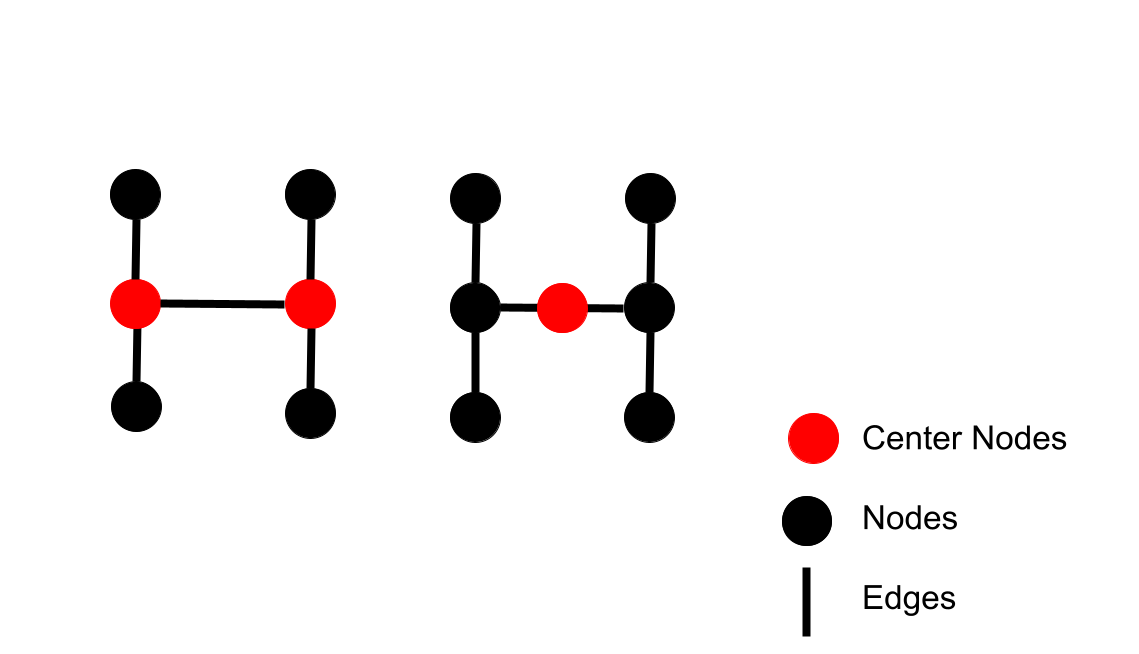
\includegraphics[width=0.5\textwidth]{images/center.png}
    \caption{Two possible representations for the reduced caterpillar graph}
    \label{fig:smallcat}
\end{figure}

When considering the case where we define the center as all points on the body of the caterpillar graph, we arrive at the following definitions:

\begin{definition}
     We define the \textbf{center body} of a reduced caterpillar graph as the following set:
        \begin{equation*}
            C := M - L
        \end{equation*}
\end{definition}

\begin{definition}
    We define $m'_w(X)$ for a configuration $X$ as:
    \begin{equation*}
        m'_w(X) := w(X) - \Sigma_{i=1} ^ k min_{a \in C} d(c, x_i)
    \end{equation*}
\end{definition}

If we add a central node to the caterpillar graph, we arrive at the following definitions:

\begin{definition}
    We define the \textbf{center node} of a reduced caterpillar graph as an additional node that receives no requests, and is labeled $c'$. Additionally, it is connected only to the two nodes closest to the middle in the center body of the graph (if there are an even number of body nodes), with weights of $0.5$. If the body is of odd length, then the node in the middle of the body is designated the center node.
\end{definition}

\begin{definition}
    We define $m''_w(X)$ for a configuration $X$ as:
    \begin{equation*}
        m''_w(X) := w(X) - \Sigma_{i=1} ^ k d(c', x_i)
    \end{equation*}
\end{definition}

We now attempt to rewrite the potential, as is done for the Multiray space. The parallel to lemma~\ref{lem:leaf2} follows in a similar manner, as for both $m'_w(X)$ and $m''_w(X)$ we can always push a point $x \in X$ to a leaf, by increasing the work done by at most the distance to the center.

We can now attempt to rewrite the potential function using these two interpretations of the "center". We consider the case where the center is the entire body of the caterpillar graph. We have:

\begin{equation*}
    \begin{split}
    w(\bar{l^i}, x_{i+1}, ..., x_k) &= min_{x_{i+1}, ..., x_k \subseteq X_i} w(X) + \Sigma_{j=1}^i d(x_j, \bar{l})\\
    &= min_{x_{i+1}, ..., x_k \subseteq X_i} w(X) + i\Delta - \Sigma_{j=1}^i d(x_j, l)
    \end{split}
\end{equation*}

We can again achieve this minimum with $X-x_{i+1}, ..., x_k\subseteq L-l$. We now must say something about the distance between the specific leaf node $l$ and the arbitrary leaf node $x_j$. The issue we encounter is that the distance between any two leaf nodes is not constant, as it is in the Multiray space. We know that $2 \leq d(l, x_j) \leq 3$, but we cannot say anything more specific. 

If we attempt to have the center point be in the middle of the body, then we run into earlier issues as there is no requirement for the path between two leaf nodes to pass through the center node. This is demonstrated in the following figure:

\begin{figure}[H]
    \centering
    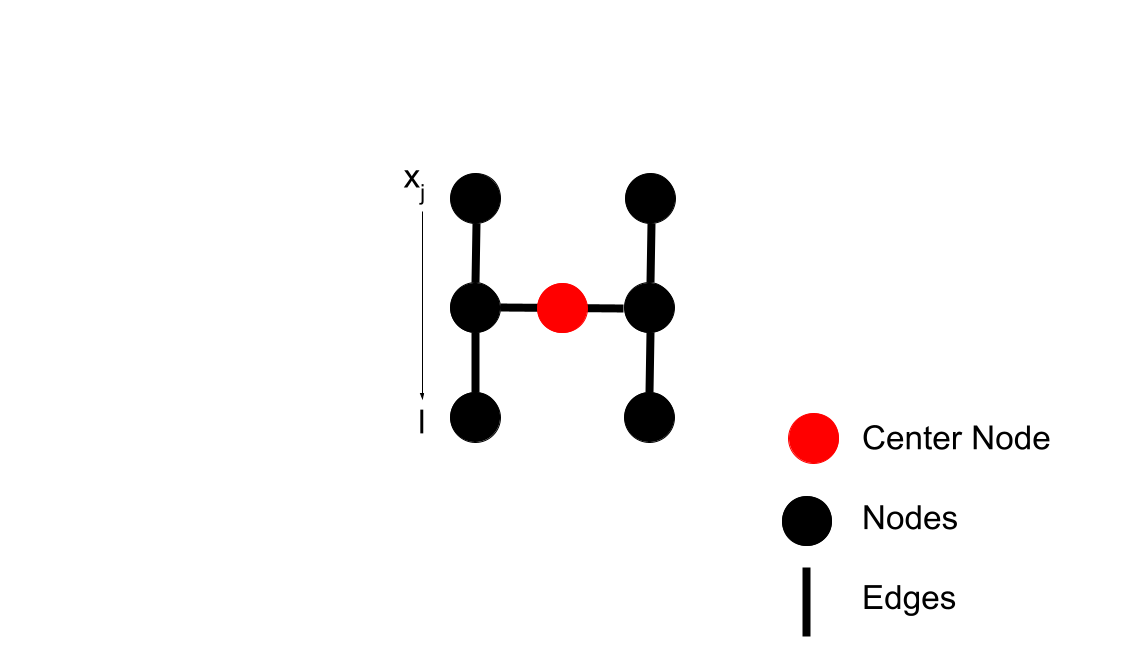
\includegraphics[width=0.5\textwidth]{images/center2.png}
    \caption{An example reduced caterpillar graph with a central node}
\end{figure}

Reverting to the case where the entire body is considered as the center, we can therefore get an inequality for our potential function, but this breaks any symetry proof we might have. We can write the potential function as follows:

\begin{equation*}
    \begin{split}
        &k^2 + \Sigma_{i=0}^k min_{l_{i+1}, ..., l_k \subseteq X_i : X_i - l_{i+1}, ..., l_k \subseteq L - l_i} \{ m_w(X_i)\} \\
        &\leq \Phi_{l_1, ..., l_k} (w)  \\
        &\leq \frac{k(3k+1)}{2} + \Sigma_{i=0}^k min_{l_{i+1}, ..., l_k \subseteq X_i : X_i - l_{i+1}, ..., l_k \subseteq L - l_i} \{ m_w(X_i)\}
    \end{split}
\end{equation*}

Continuing the proof from here yields no useful results, as we have been unable to show that the potential function is symmetric under permutations of the leaf nodes.